% Appendix A

\chapter{Simulink Controllers} % Main appendix title

\label{AppendixB} % For referencing this appendix elsewhere, use \ref{AppendixB}

\lhead{Appendix A. \emph{Simulink Controllers}} % Change X to a consecutive letter; this is for the header on each page - perhaps a shortened title


This appendix documents the simulink controllers developed in chapters \ref{Chapter3} and \ref{Chapter4}. The subsections below include images of the controllers as well as brief descriptions of the Simulink blocks and their functions.

%----------------------------------------------------------------------------------------
%	SECTION 1
%----------------------------------------------------------------------------------------

\section{Baseline NREL 5-MW Feedback Control.} \label{sectionB-1}

The figures in this section illustrate the Simulink model used to simulate the Upwind Turbine in chapters \ref{Chapter3} and \ref{Chapter4}. The Simulink systems shown below model an NREL 5-MW turbine with the control system described in the NREL 5-MW specification\cite{jonkman2009}. Figure \ref{figB-1} shows the top level Simulink system. The green box contains a version of FAST that has been specially compiled to interact with Simulink control systems. At each time step this version of FAST takes generator torque, generator power, yaw position, and blade pitch as inputs. The FAST outputs are defined by the input file \textit{primary.fst}. A typical set of outputs can be seen in Appendix \ref{AppendixA}. All of the yellow boxes shown in the figures below record simulation data and write it to output files at each time step. At each time step, generator speed is extracted from the FAST output and passed through a low pass filter (the small blue box in Figure \ref{figB-1}) to remove high frequency oscillations. This filtered generator speed is then fed to the pitch and torque controllers (the two largest blue boxes), which determine the blade pitch, generator torque, and generator power inputs to FAST. The Yaw position input is specified by the Yaw controller (the grey box), but in this case the yaw controller simply specifies a constant value of 0\degree.

 \begin{figure}[ht]
	\centering
		\includegraphics[width=\linewidth]{Figures/AppendixBFigures/baseline1.png}
	\caption{Top level Simulink system for model of NREL 5-MW with baseline (no feed forward) control.}
	\label{figB-1}
\end{figure}

Figure \ref{figB-2} shows the Pitch Controller subsystem. It takes filtred generator speed and current blade pitch angle as inputs. The NREL 5-MW turbine uses a nonlinear Proportional and Integral (PI) controller for pitch control. In this control scheme the control gains are a function of blade pitch. The Gain Schedule subsystem uses the current blade pitch to adjust the proportional (Kp) and Integral (Ki) control gains using the logic shown in Figure \ref{figB-3}. The filtered generator speed is compared to the rated generator speed to determine the generator speed error. The Total Pitch Command subsystem takes the generator speed error and adjusted control gains as inputs then applies PI control using the logic shown in Figure \ref{figB-4} to produce a blade pitch command. That blade pitch command is fed through the Blade Pitch Actuator block, which is a 2nd order model of the blade pitch actuator dynamics with a natural frequency of 1 Hz and a damping ratio of 0.7, to produce the pitch command that will be input to FAST. The Blade Pitch Actuator block is included here because FAST does not model blade pitch actuator dynamics.

 \begin{figure}[ht]
	\centering
		\includegraphics[width=\linewidth]{Figures/AppendixBFigures/baseline2.png}
	\caption{Pitch Controller subsystem for Simulink model of NREL 5-MW with baseline control.}
	\label{figB-2}
\end{figure}

 \begin{figure}[ht]
	\centering
		\includegraphics[width=\linewidth]{Figures/AppendixBFigures/baseline3.png}
	\caption{Gain Schedule subsystem for Simulink model of NREL 5-MW with baseline control.}
	\label{figB-3}
\end{figure}

 \begin{figure}[ht]
	\centering
		\includegraphics[width=\linewidth]{Figures/AppendixBFigures/baseline4.png}
	\caption{Total Pitch Command subsystem for Simulink model of NREL 5-MW with baseline control.}
	\label{figB-4}
\end{figure}

Figure \ref{figB-5} shows the Torque Controller subsystem.  It takes filtred generator speed, current blade pitch angle, and unfiltered generator speed as inputs. The embedded Matlab function GenTorque uses blade pitch angle to determine if the turbine is in region 3 control. It then calculates the appropriate generator torque for the current filtered generator speed and control region. The full text of GenTorque is shown in Figure \ref{figB-6}. The generator torque command is passed through value and rate limiters to produce the generator torque command that will be input to FAST. To calculate generator power, the unfiltered generator speed is multiplied by the generator torque command then adjusted to account for the efficiency of the generator.

 \begin{figure}[ht]
	\centering
		\includegraphics[width=\linewidth]{Figures/AppendixBFigures/baseline5.png}
	\caption{Torque Controller subsystem for Simulink model of NREL 5-MW with baseline control.}
	\label{figB-5}
\end{figure}


\begin{figure}[ht]
	\centering
%\noindent
		\includegraphics[width=\linewidth]{Figures/AppendixBFigures/baseline9.png}
	\caption{Embedded Matlab function GenTorque for baseline control.}
	\label{figB-6}
\end{figure}


%\FloatBarrier

%----------------------------------------------------------------------------------------
%	SECTION 2
%----------------------------------------------------------------------------------------

\section{NREL 5-MW Turbine With Feed Forward Optimal Pitch Control.} \label{sectionB-2}
The figures in this section illustrate the Simulink model used to simulate A Downwind turbine with feed forward optimum pitch control. This is the feed forward controller analyzed in Chapter \ref{Chapter3}. Figure \ref{figB-7} shows the top level Simulink system. Much of the figure looks similar to Figure \ref{figB-1}, which illustrates the baseline (or upwind) turbine. In fact, the FAST block and all of the components of the baseline closed loop controller are present in Figure \ref{figB-7}. However, there is a new component. In the lower left corner there is a Feed Forward Controller subsystem that sends a FF Pitch Command signal to the Pitch Controller subsystem.

 
 
\begin{figure}[ht]
	\centering
		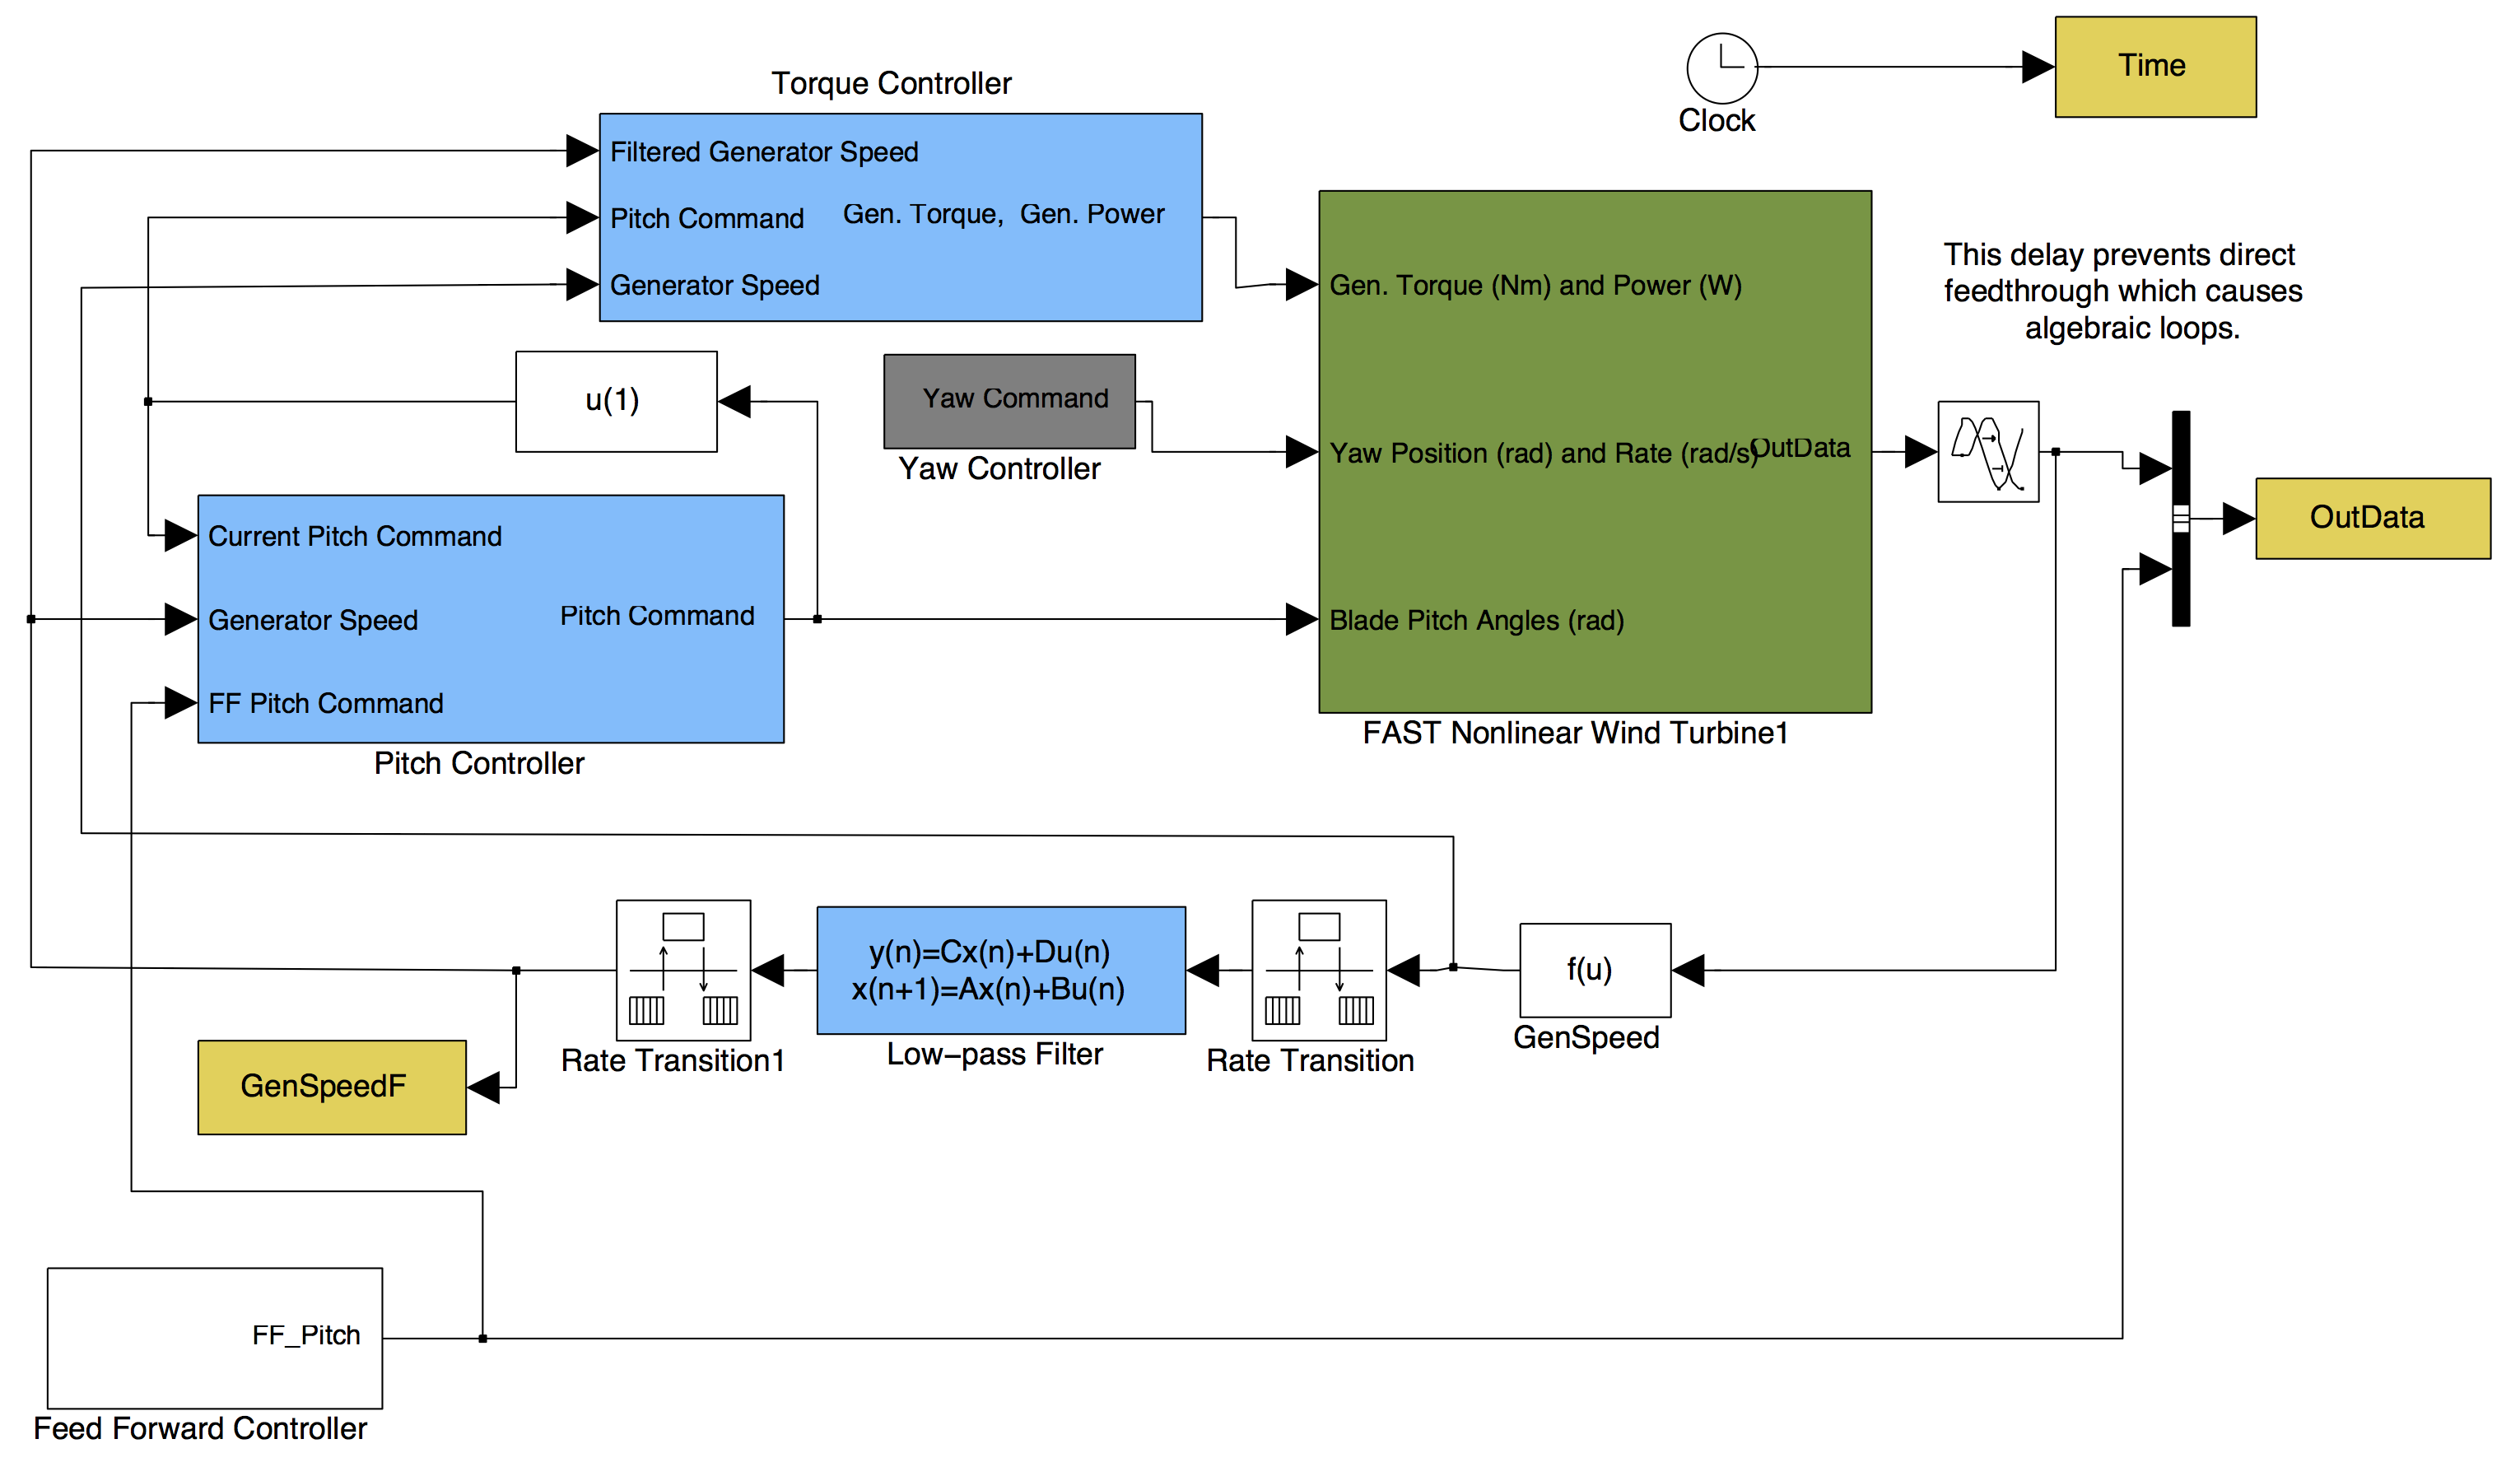
\includegraphics[width=\linewidth]{Figures/AppendixBFigures/FF_Pitch1.png}
	\caption{Top level Simulink system for model of NREL 5-MW with feed forward optimal pitch control.}
	\label{figB-7}
\end{figure}

Figure \ref{figB-8} shows the Feed Forward Controller subsystem. This subsystem is simple because most of the calculations are done prior to the simulation by a set of Matlab files. The FF Dynamic Wind Speed Lookup block contains a time history of the dynamic feed forward velocity ($U_{ff}$), which has been generated based on the output data from the Upwind Turbine simulation. Dynamic feed forward velocity is described in Section \ref{section3-3-3} and Equation \ref{eq3-3}. To save space, the Matlab files that are used to process Upwind Turbine output data and create the FF Dynamic Wind Speed Lookup table have not been included in this appendix. Those Matlab files are fairly long and several sets of files were required for the different sets of assumptions and operating conditions used in Chapter \ref{Chapter3}. The FF Pitch Lookup Table contains a table relating dynamic feed forward velocity to the corresponding optimum pitch angle that will keep the turbine at a 12.1 RPM rotor speed. The relationship between dynamic feed forward velocity and optimum pitch angle is shown in Figure \ref{fig3-11}.

\begin{figure}[ht]
	\centering
		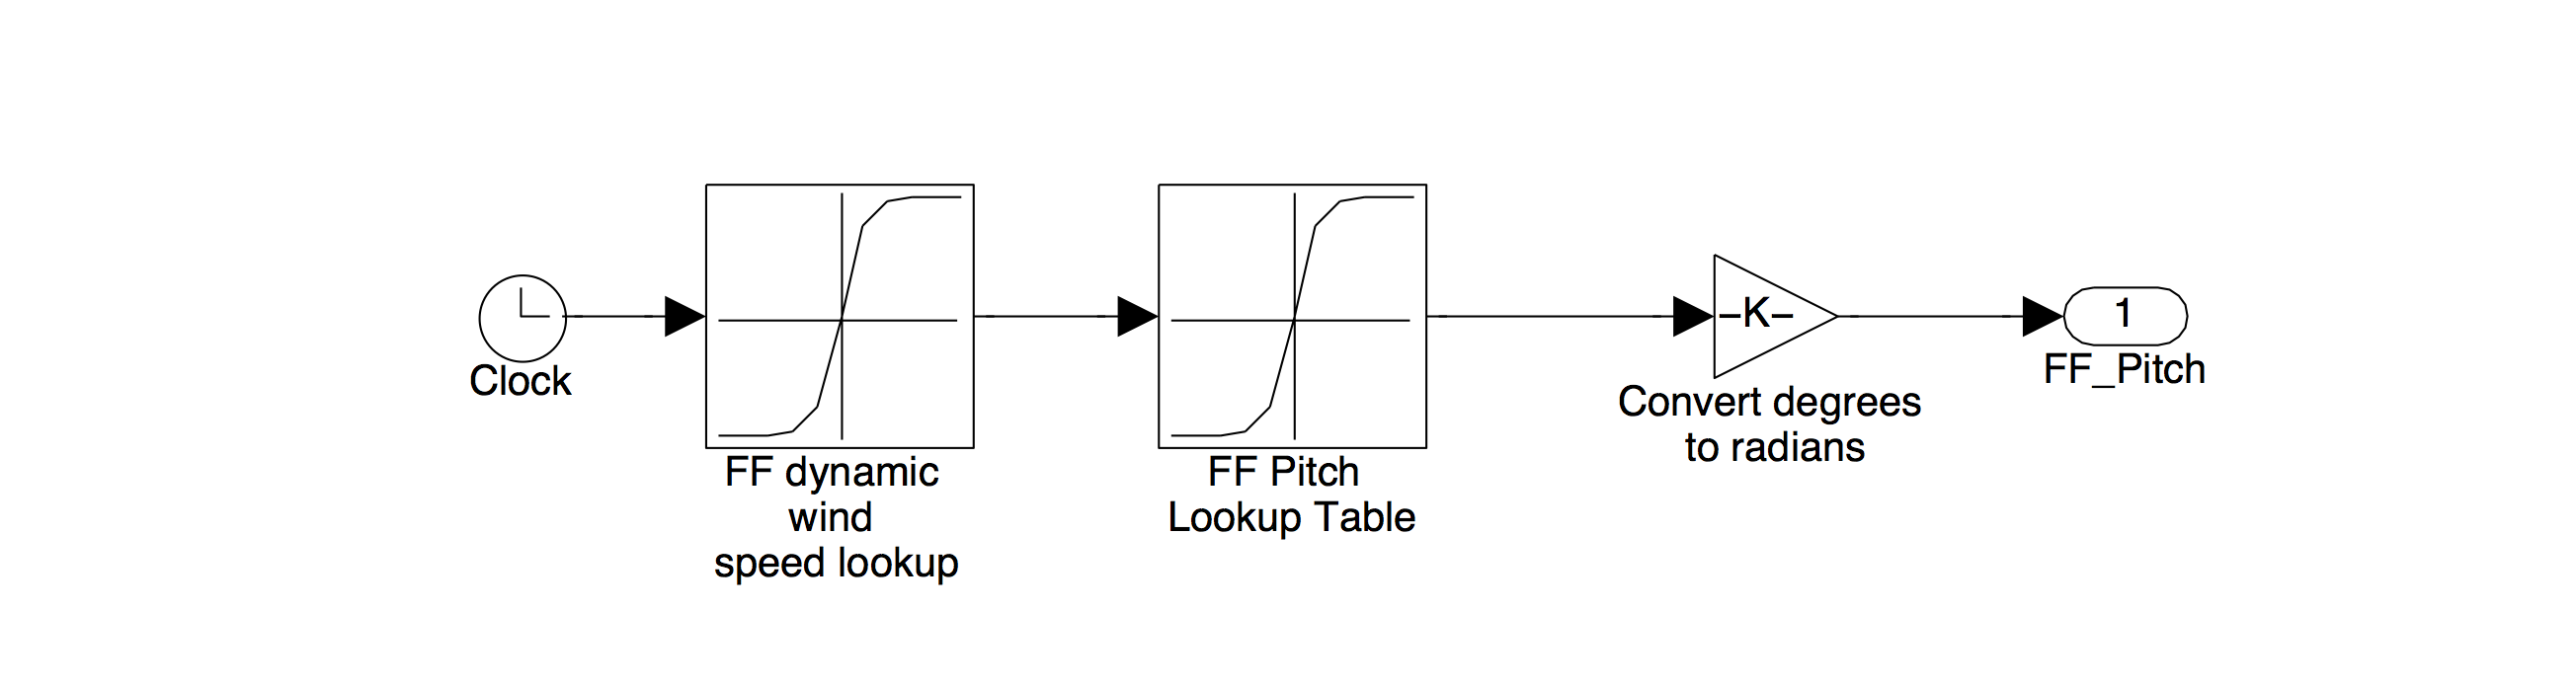
\includegraphics[width=\linewidth]{Figures/AppendixBFigures/FF_Pitch2.png}
	\caption{Feed Forward Controller subsystem for Simulink model of NREL 5-MW with feed forward optimal pitch control.}
	\label{figB-8}
\end{figure}

The Pitch Controller subsystem is shown in Figure \ref{figB-9}. It has been modified to accept the FF Pitch Command. The entire closed loop pitch control system is still present in this subsystem. The feed forward pitch is added to the Blade Pitch Command coming from the Total Pitch Command subsystem. This combined pitch command, from the closed loop controller and the feed forward controller, is then fed through the blade pitch actuator model before being passed to FAST.

\begin{figure}[ht]
	\centering
		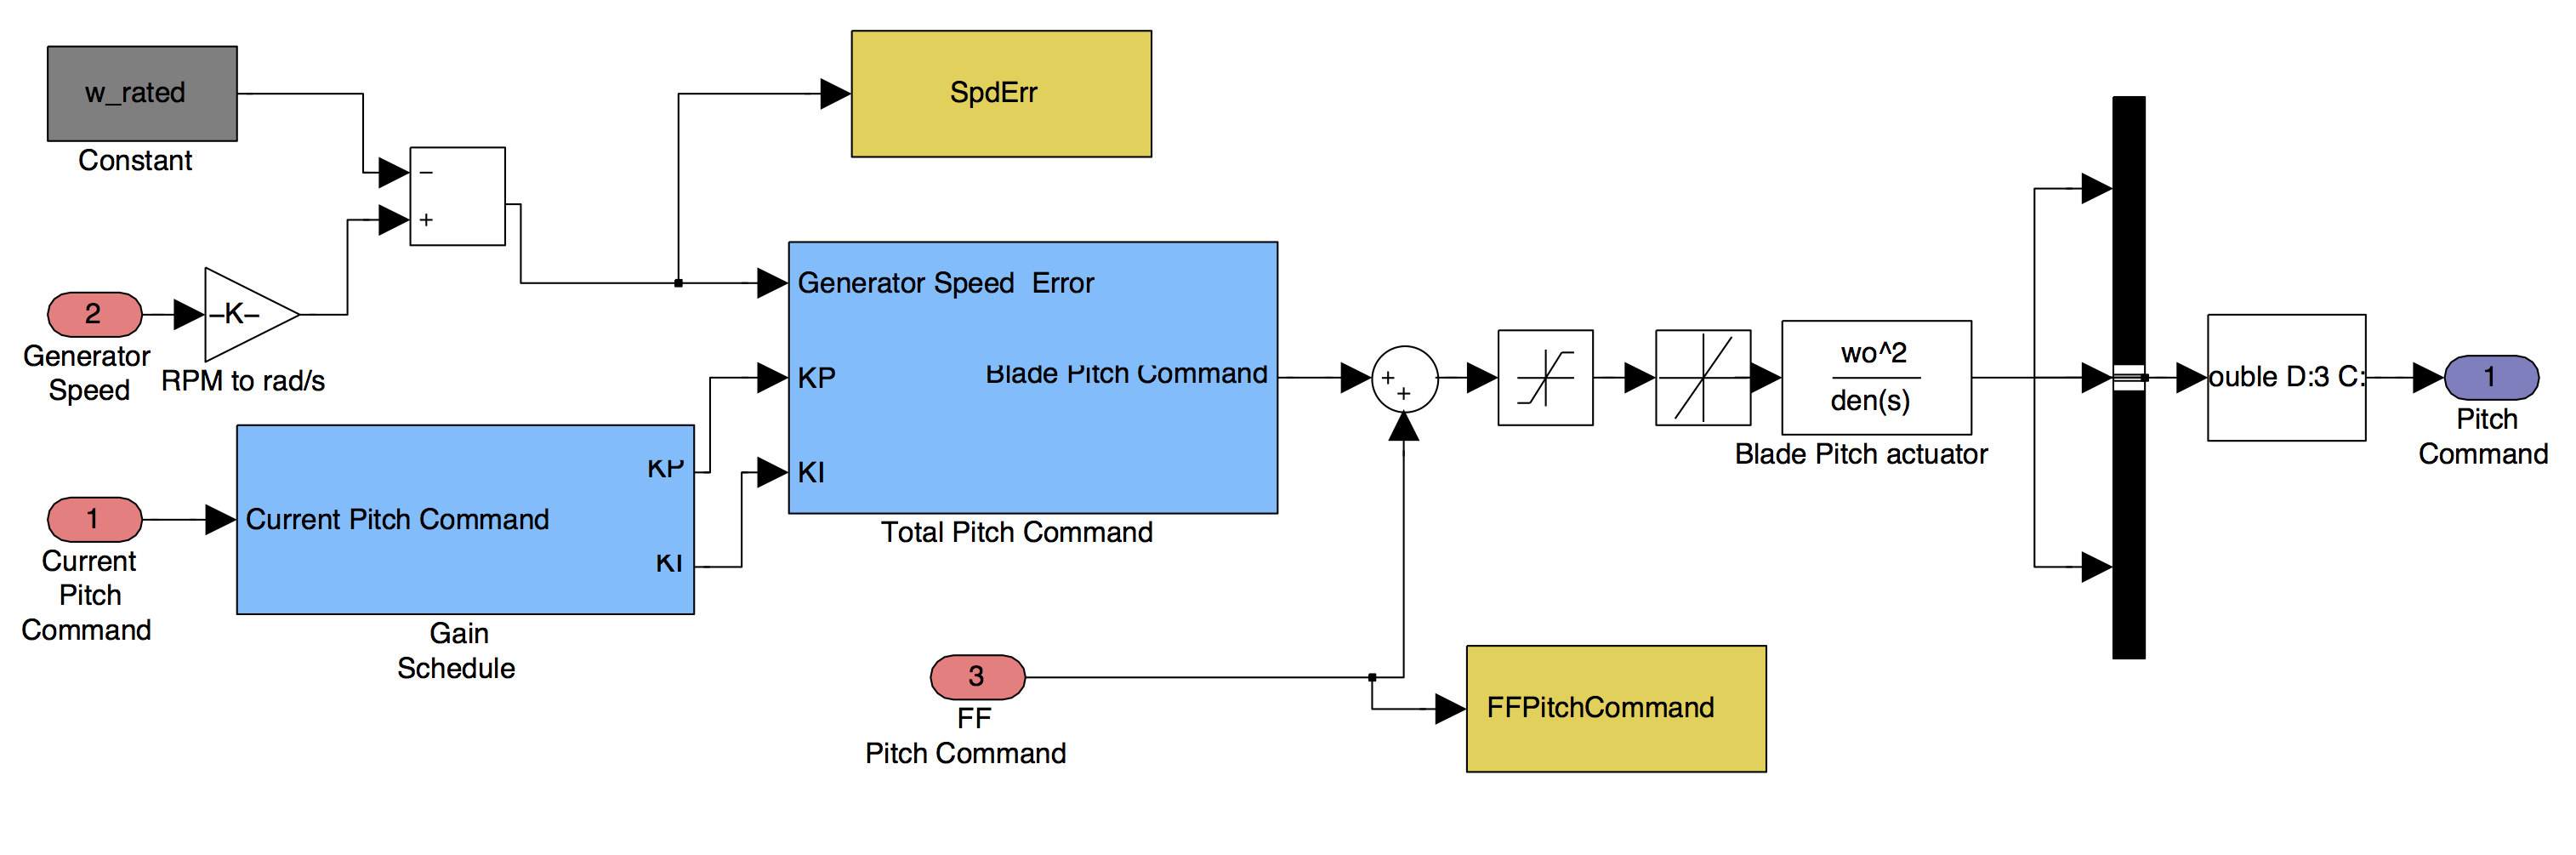
\includegraphics[width=\linewidth]{Figures/AppendixBFigures/FF_Pitch3.png}
	\caption{Pitch Controller subsystem for Simulink model of NREL 5-MW with feed forward optimal pitch control.}
	\label{figB-9}
\end{figure}

The Gain Schedule, Total Pitch Command, Torque Controller, and GenTorque subsystems are identical to the subsystems in the baseline NREL 5-MW controller, so they are not shown here. The form and function of those subsystems are described in Section \ref{sectionB-1}.


%----------------------------------------------------------------------------------------
%	SECTION 3
%----------------------------------------------------------------------------------------

\section{NREL 5-MW Turbine With Feed Forward Derating Control.} \label{sectionB-3}

The figures in this section illustrate the Simulink model used to simulate a Downwind Turbine with feed forward optimum pitch control. This is the feed forward controller analyzed in Chapter \ref{Chapter4}. Figure \ref{figB-10} shows the top level Simulink system. Much of the figure looks similar to Figure \ref{figB-1}, which illustrates the baseline (or upwind) turbine. The FAST block and all of the components of the baseline closed loop controller are present in Figure \ref{figB-10}. However,in the lower left corner there is a Feed Forward Controller subsystem that sends FF\_pwrFactor and FF\_minPit commands to the Pitch Controller and Torque Controller subsystems. FF\_pwrFactor stands for Feed Forward Power Factor which is a measure of the turbine's current rated capacity as a fraction of full rated capacity. For example, a turbine in normal operation would have a power factor of 1. A turbine that has been derated by 20\% would have a power factor of 0.8. FF\_minPitch stands for Feed Forward Minimum Pitch. The minimum pitch is a function of the power factor, but it was easiest to implement it as a separate signal here. The minimum pitch is used to derate a turbine operating in region 2 control.

 \begin{figure}[ht]
	\centering
		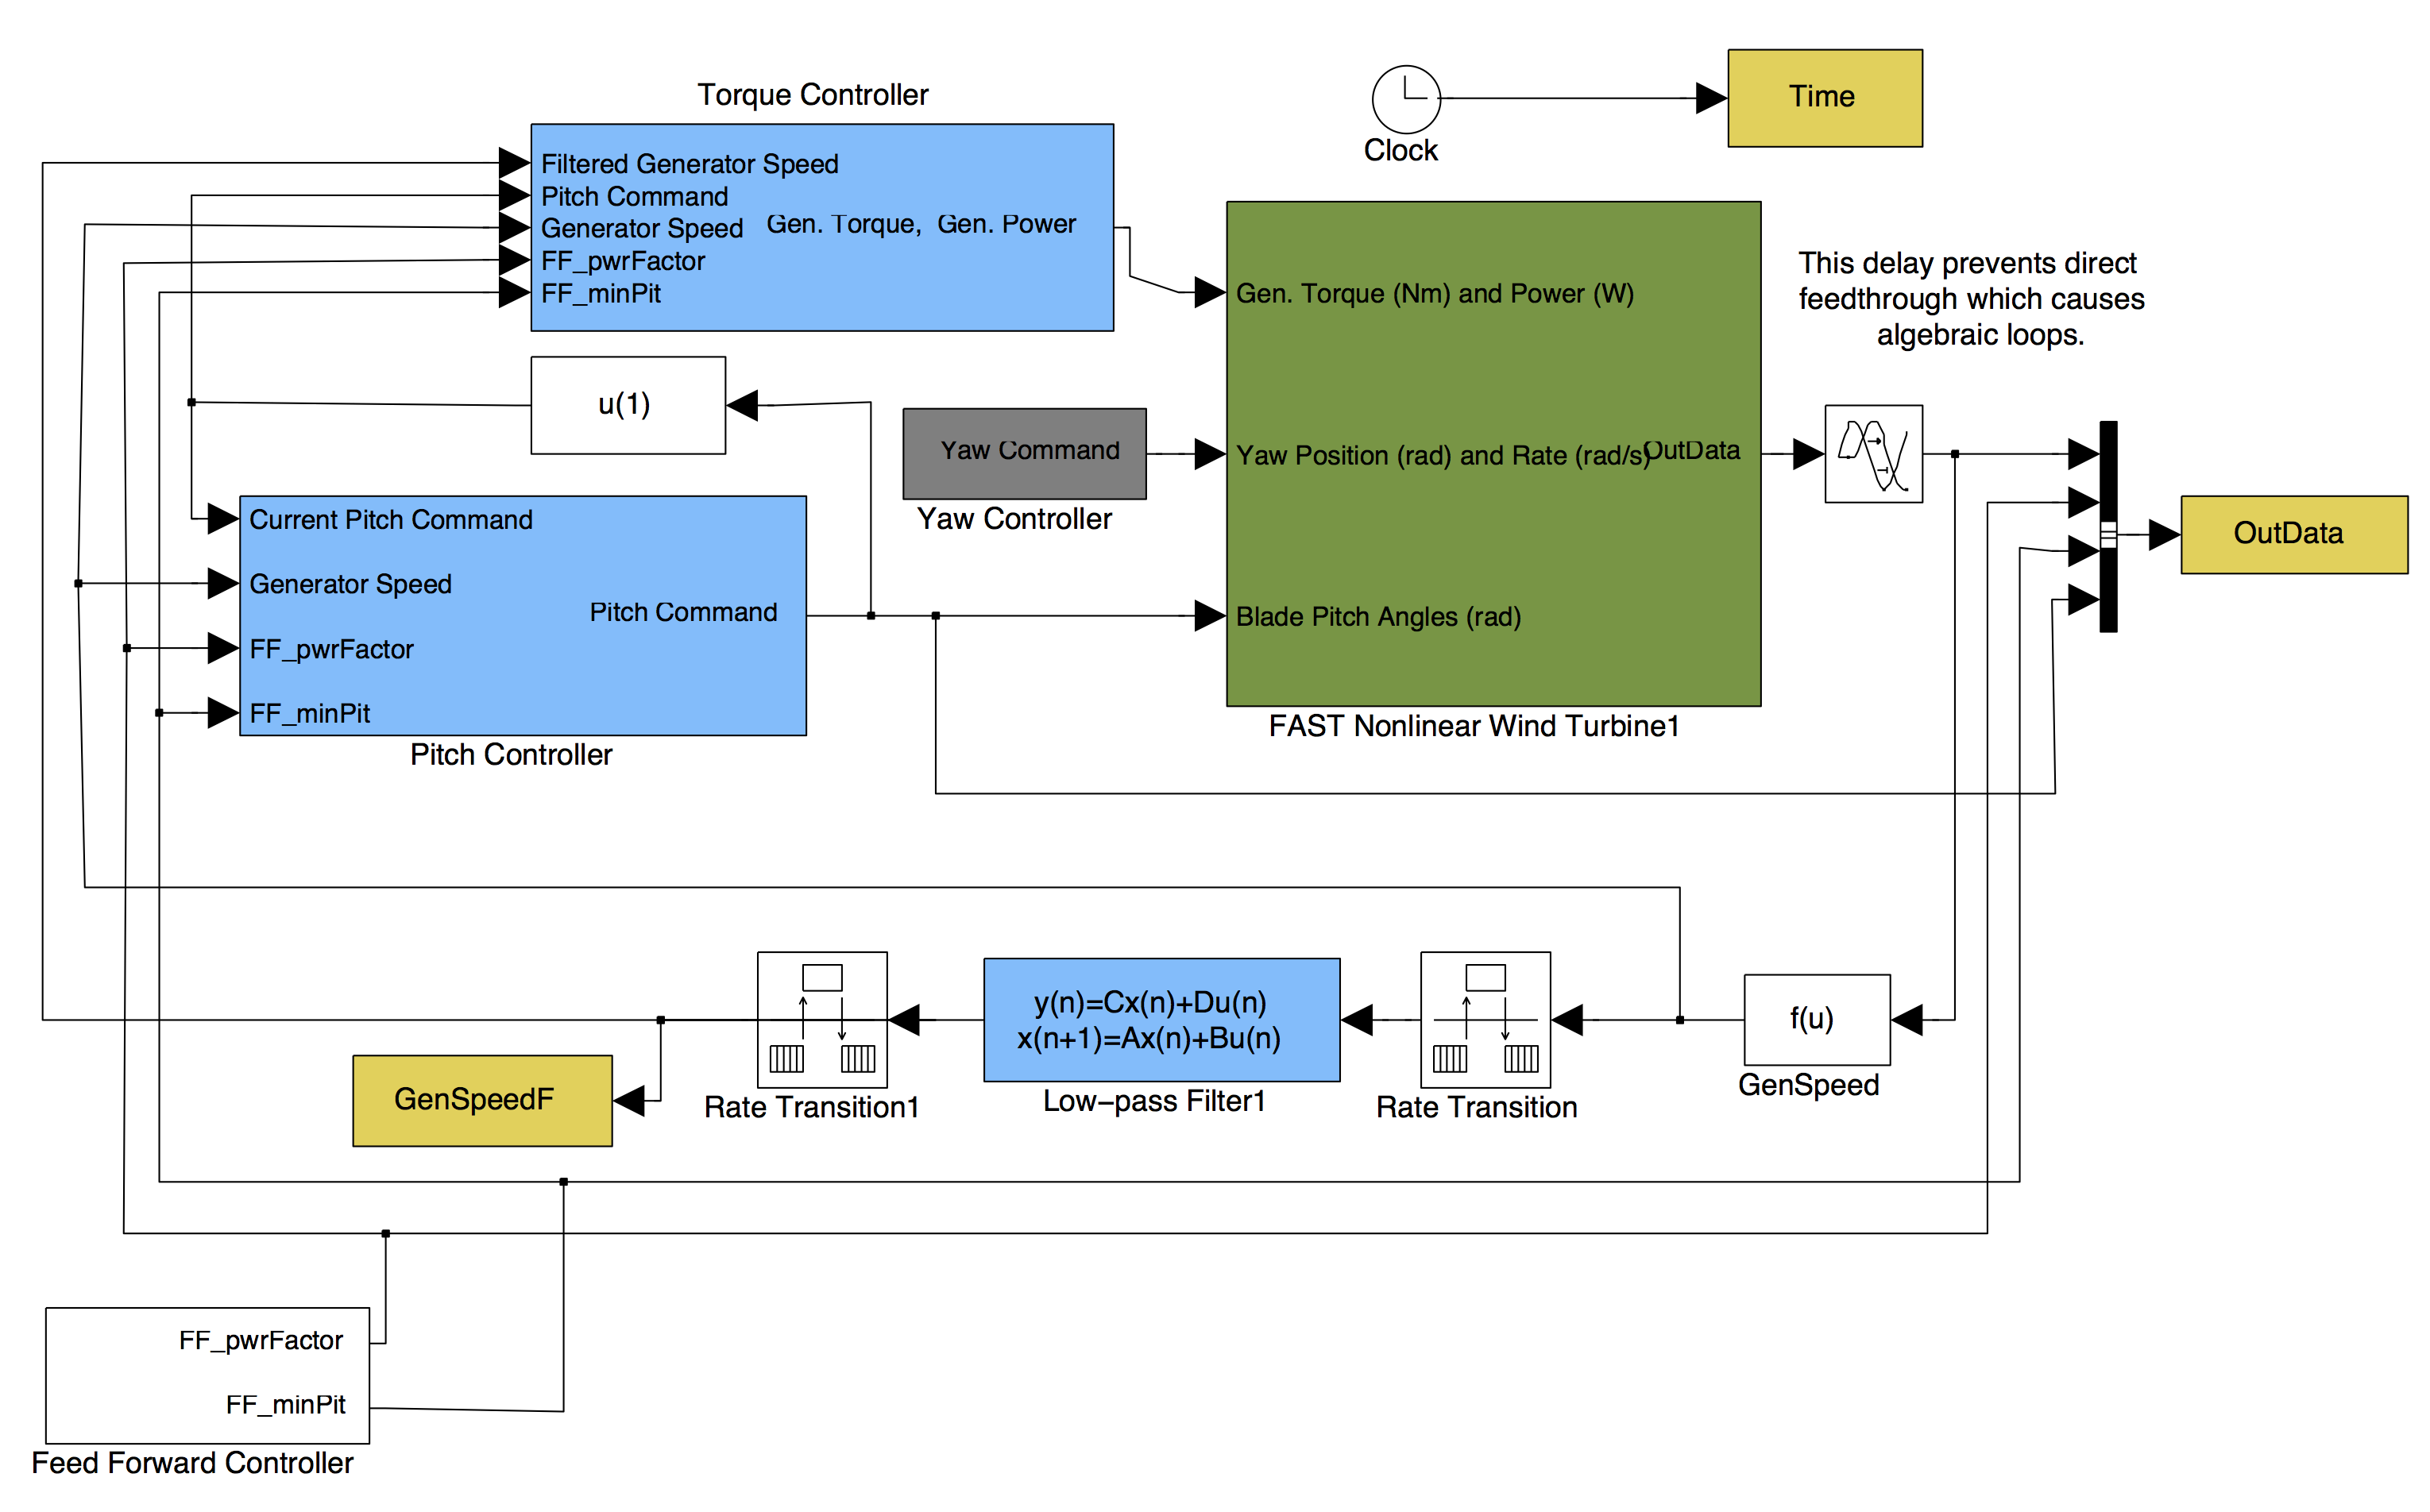
\includegraphics[width=\linewidth]{Figures/AppendixBFigures/FF_Derate1.png}
		
	\caption{Top level Simulink system for model of NREL 5-MW with feed forward derating control.}
	\label{figB-10}
\end{figure}

Figure \ref{figB-11} shows the Feed Forward Controller subsystem. The FF Derate Factor Lookup Table block contains a time history of the derate factor, which has been generated based on the output data from the Upwind Turbine simulation. The derate factor is the amount of derating requested by the feed forward controller (as a fraction of full turbine capacity). Most of the time the derate factor is 0, but it is increased when the turbine is derated. The derate factor signal is fed through the Low Pass Filter block to prevent abrupt changes in turbine rating (as discussed in Section \ref{section4-4}). Subtracting the derate factor from 1 turns it into a power factor signal. The Min Pitch Lookup Table block determines the minimum pitch corresponding to the current power factor. Finaly, the FF\_pwrFactor and FF\_minPit signals are then passed out of the controller.

\begin{figure}[ht]
	\centering
		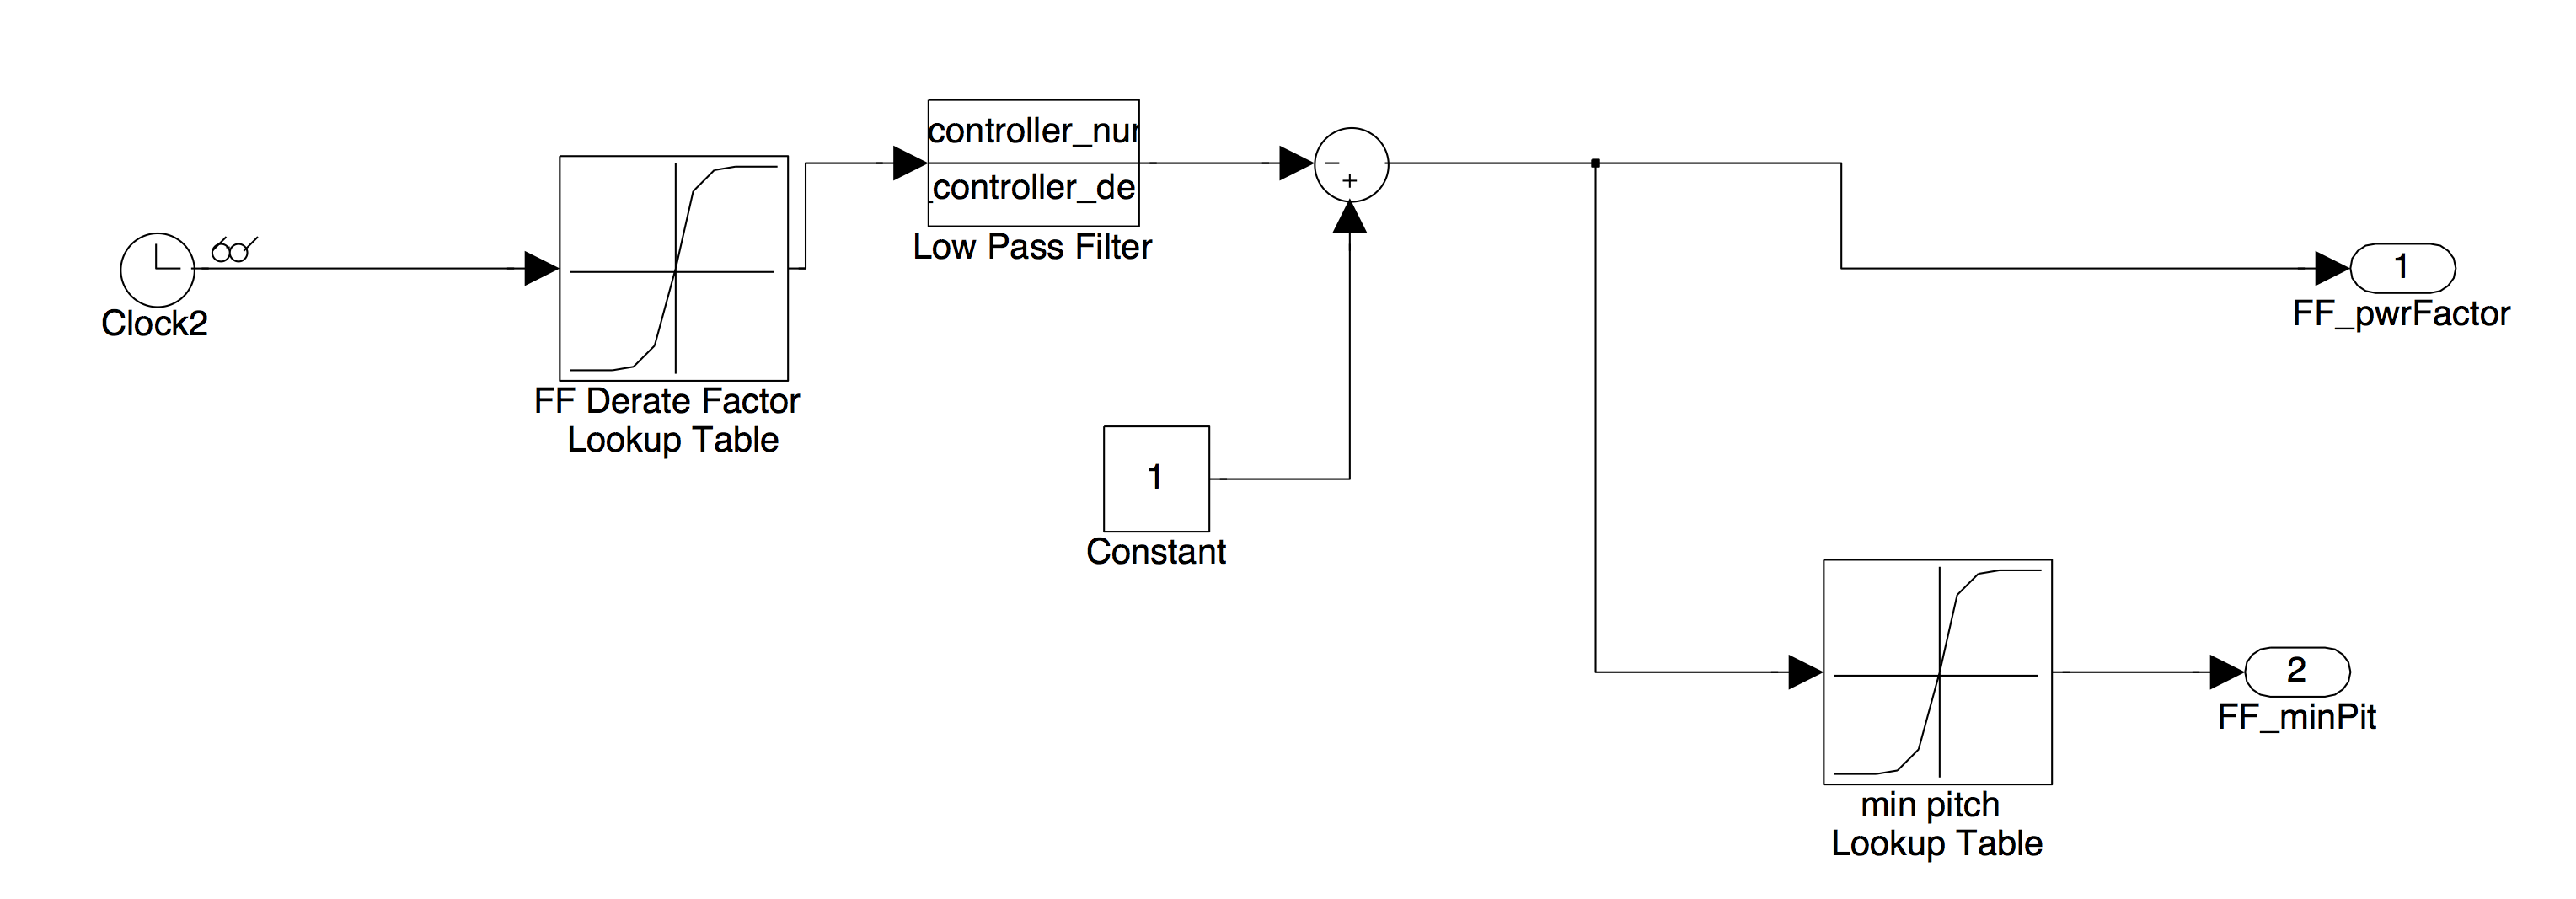
\includegraphics[width=\linewidth]{Figures/AppendixBFigures/FF_Derate2.png}
	\caption{Feed Forward Controller subsystem for Simulink model of NREL 5-MW with feed forward derating control.}
	\label{figB-11}
\end{figure}

The Pitch Controller subsystem is shown in Figure \ref{figB-12}. It has been modified to accept the FF\_pwrFactor and FF\_minPit commands. The rated generator speed (GenSpRef) is multiplied by the power factor (FF\_pwrFactor). When the turbine is derated, and the power factor is less than 1, this reduces the generator speed that the turbine pitch controller is attempting to track. The minimum pitch (FF\_minPit) is passed to the Total Pitch Command block. The Gain Schedule block is identical to the PI Control Gain Adjustment block described by Section \ref{sectionB-1} and Figure \ref{figB-3}. It will not be described here. 

\begin{figure}[ht]
	\centering
		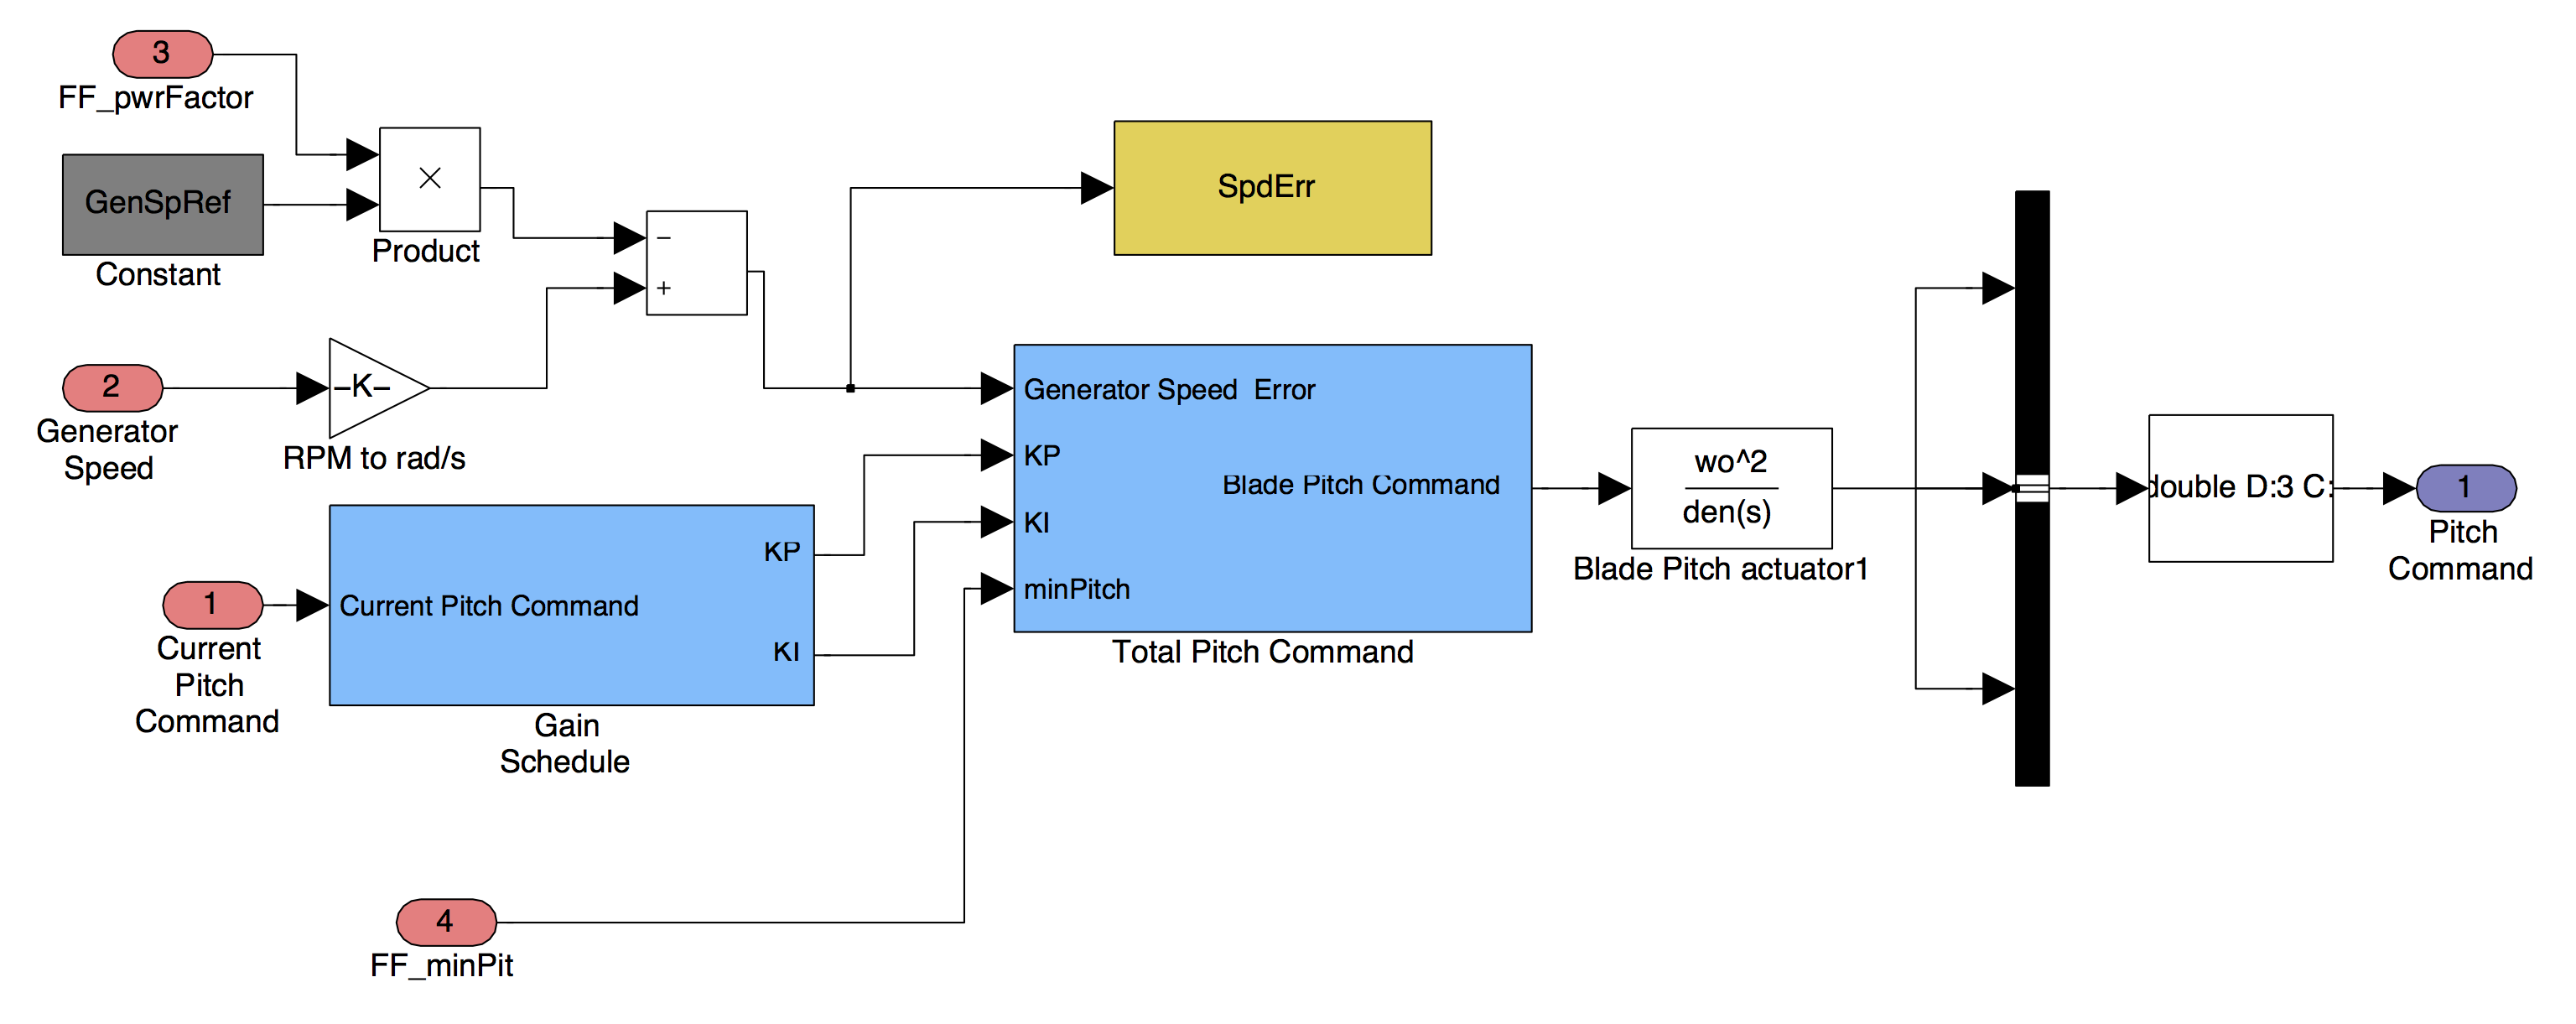
\includegraphics[width=\linewidth]{Figures/AppendixBFigures/FF_Derate3.png}
	\caption{Pitch Controller subsystem for Simulink model of NREL 5-MW with feed forward derating control.}
	\label{figB-12}
\end{figure}

The Total Pitch Command subsystem is shown in Figure \ref{figB-13}. This subsystem applies nonlinear PI control, much like it does in the baseline controller (Figure \ref{figB-4}). However, this subsystem uses the minimum pitch signal (minPitch)  as the lower bounds for blade pitch control. The baseline controller uses 0\degree{} as the lower bounds.

\begin{figure}[ht]
	\centering
		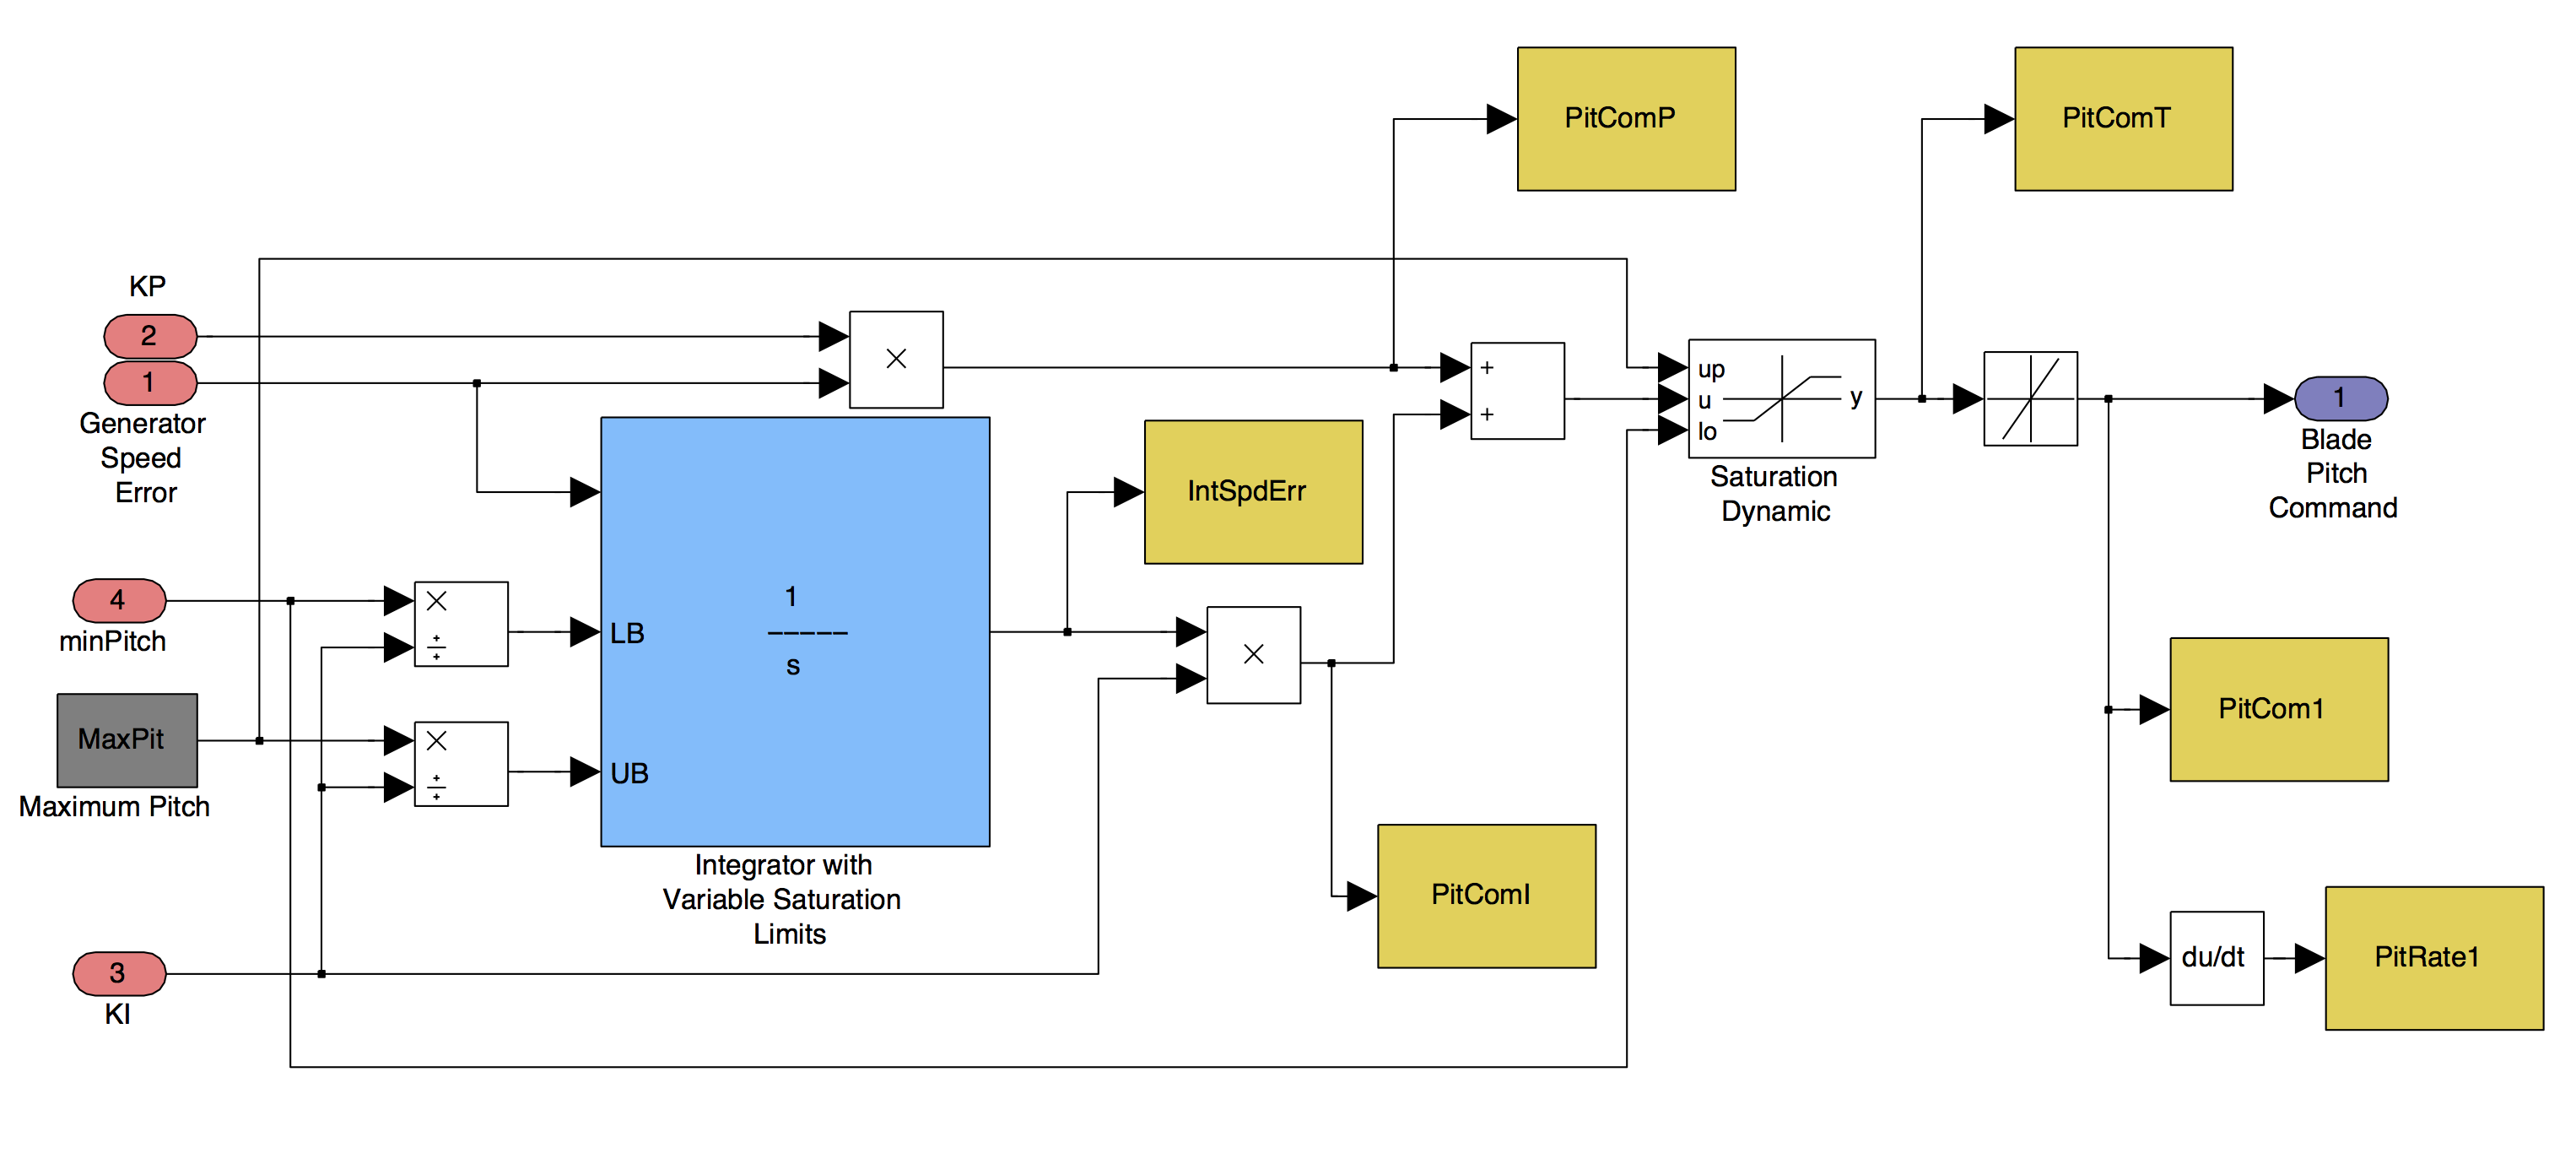
\includegraphics[width=\linewidth]{Figures/AppendixBFigures/FF_Derate5.png}
	\caption{Total Pitch Command subsystem for Simulink model of NREL 5-MW with feed forward derating control.}
	\label{figB-13}
\end{figure}

Figure \ref{figB-14} shows the Torque Controller subsystem. Much of this subsystem remains unchanged from the baseline controller. The power factor (FF\_pwrFactor) and minimum blade pitch (FF\_minPit) commands are passed to the embedded Matlab function GenTorque along with the filtered generator speed and current pitch command. The full text of GenTorque is shown in Figure \ref{figB-15}. GenTorque uses the derate factor to adjust the shapes of the NREL 5-MW torque-speed curves when the turbine is derated. It then compares the current pitch command to the minimum pitch to determine if the turbine is in region 3 control. Finally, it calculates the appropriate generator torque for the current filtered generator speed, control region, and derate factor.

\begin{figure}[ht]
	\centering
		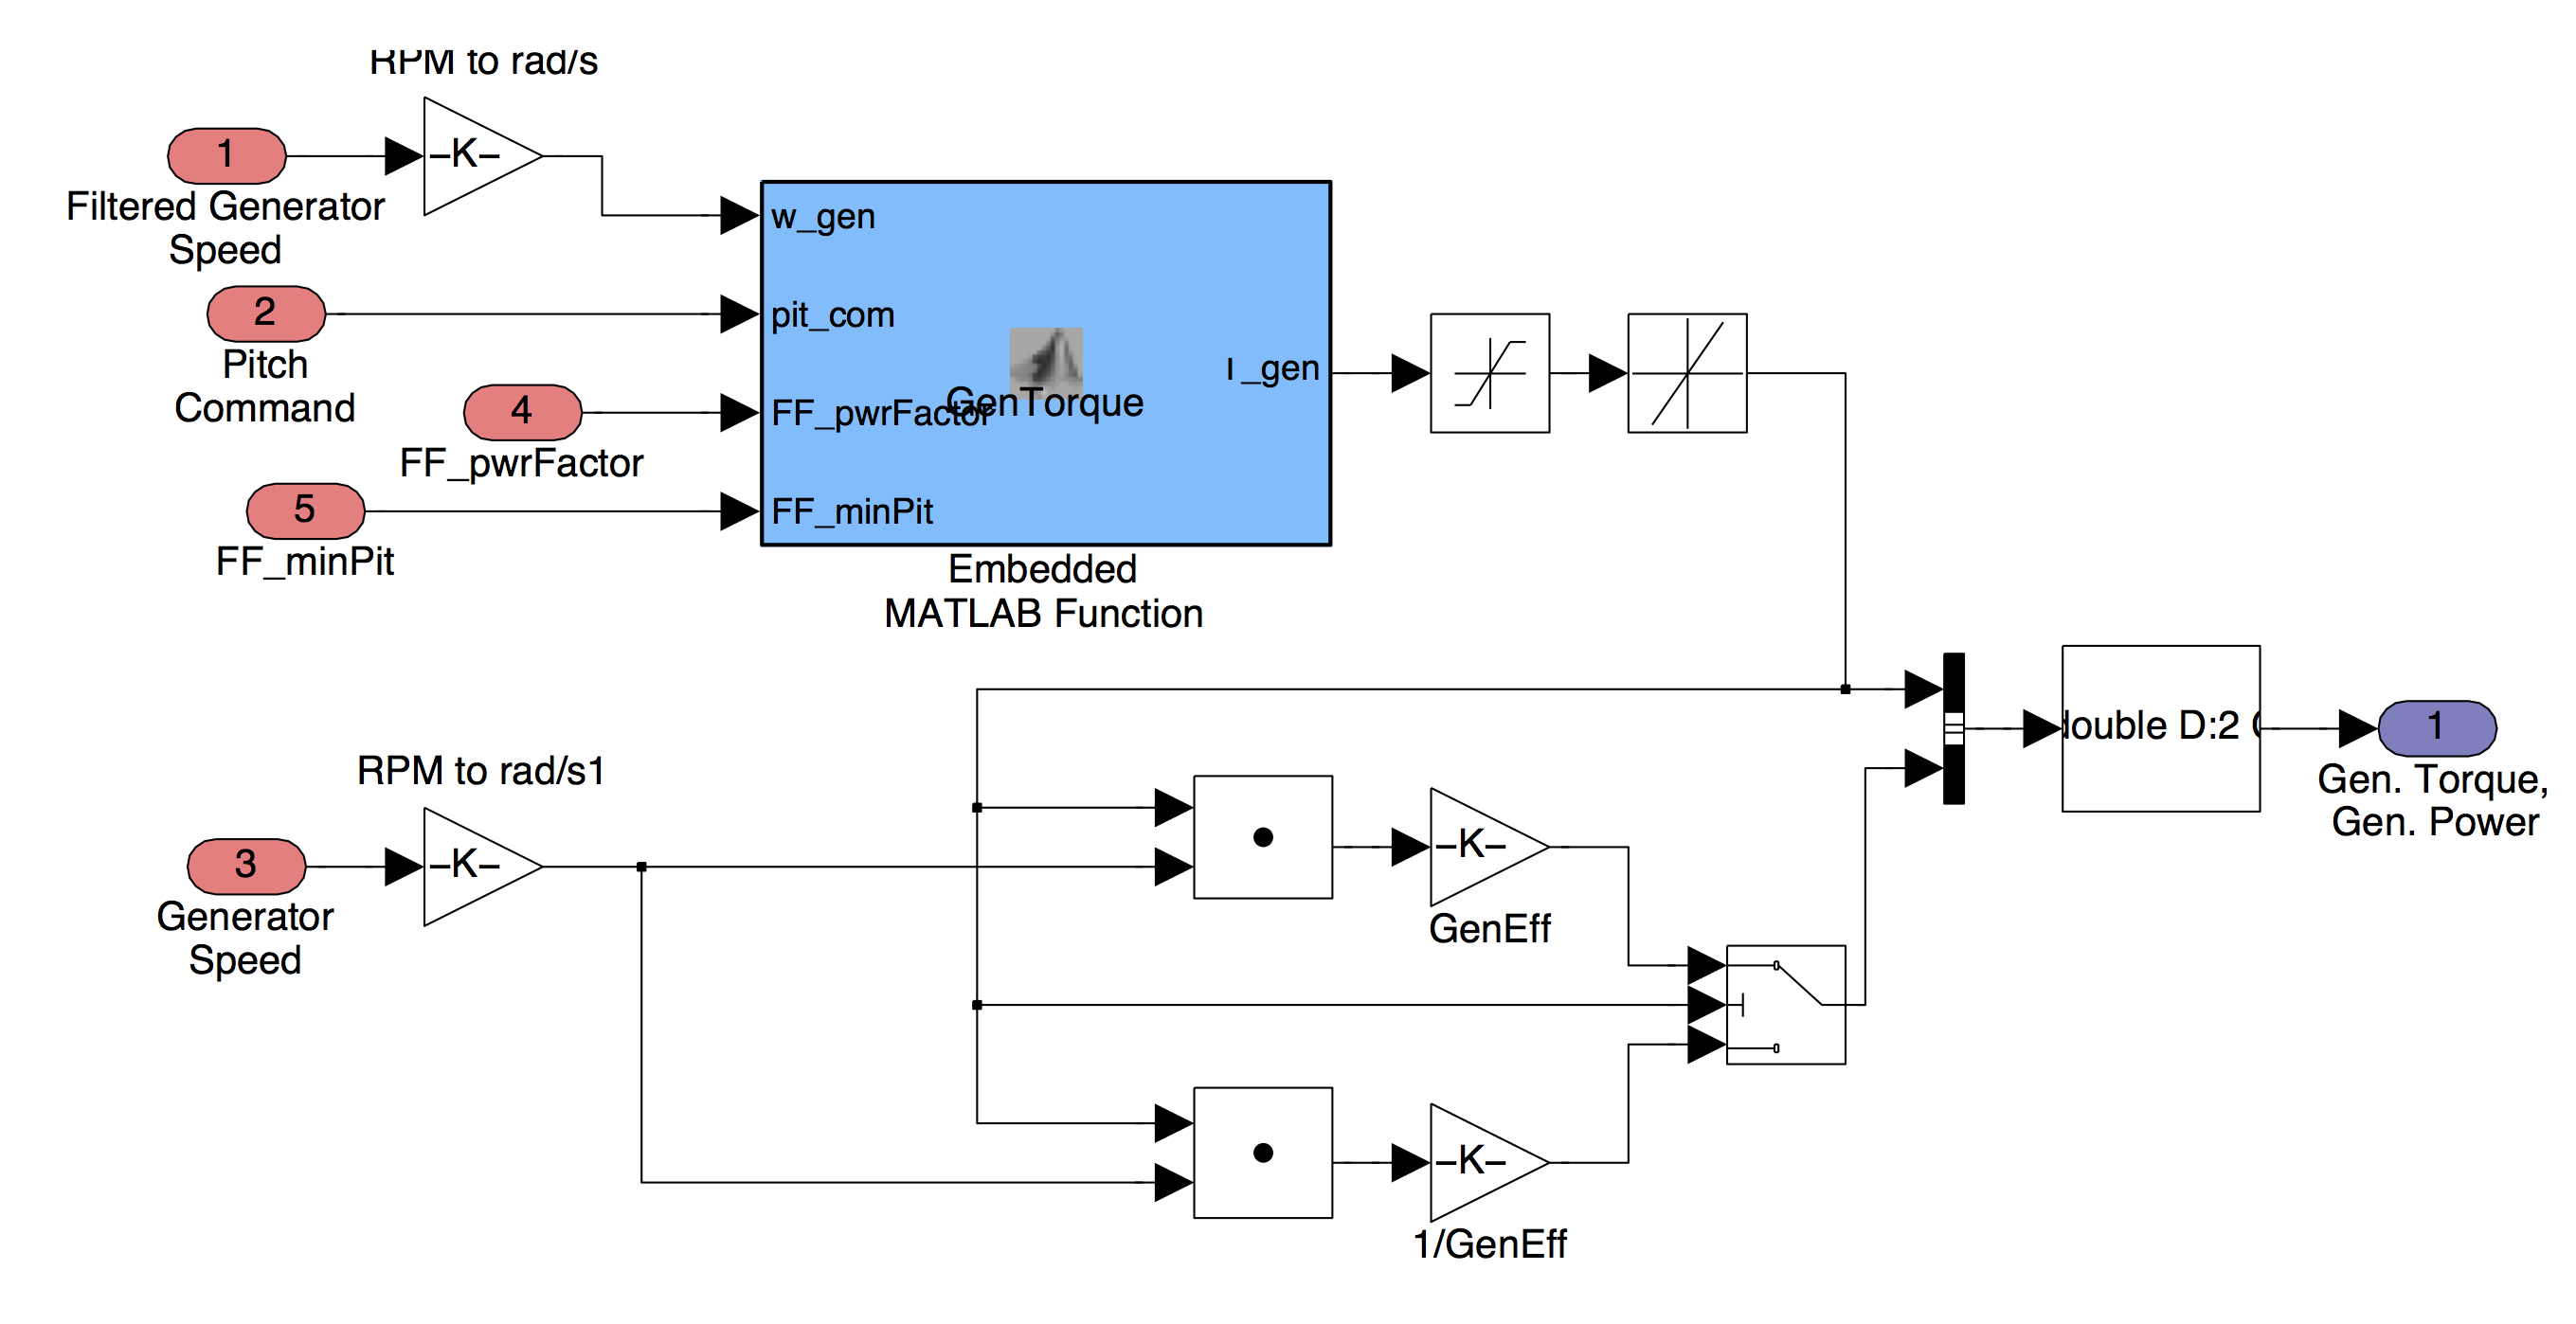
\includegraphics[width=\linewidth]{Figures/AppendixBFigures/FF_Derate6.png}
	\caption{Torque Controller subsystem for Simulink model of NREL 5-MW with feed forward derating control.}
	\label{figB-14}
\end{figure}

 \begin{figure}[ht]
	\centering
		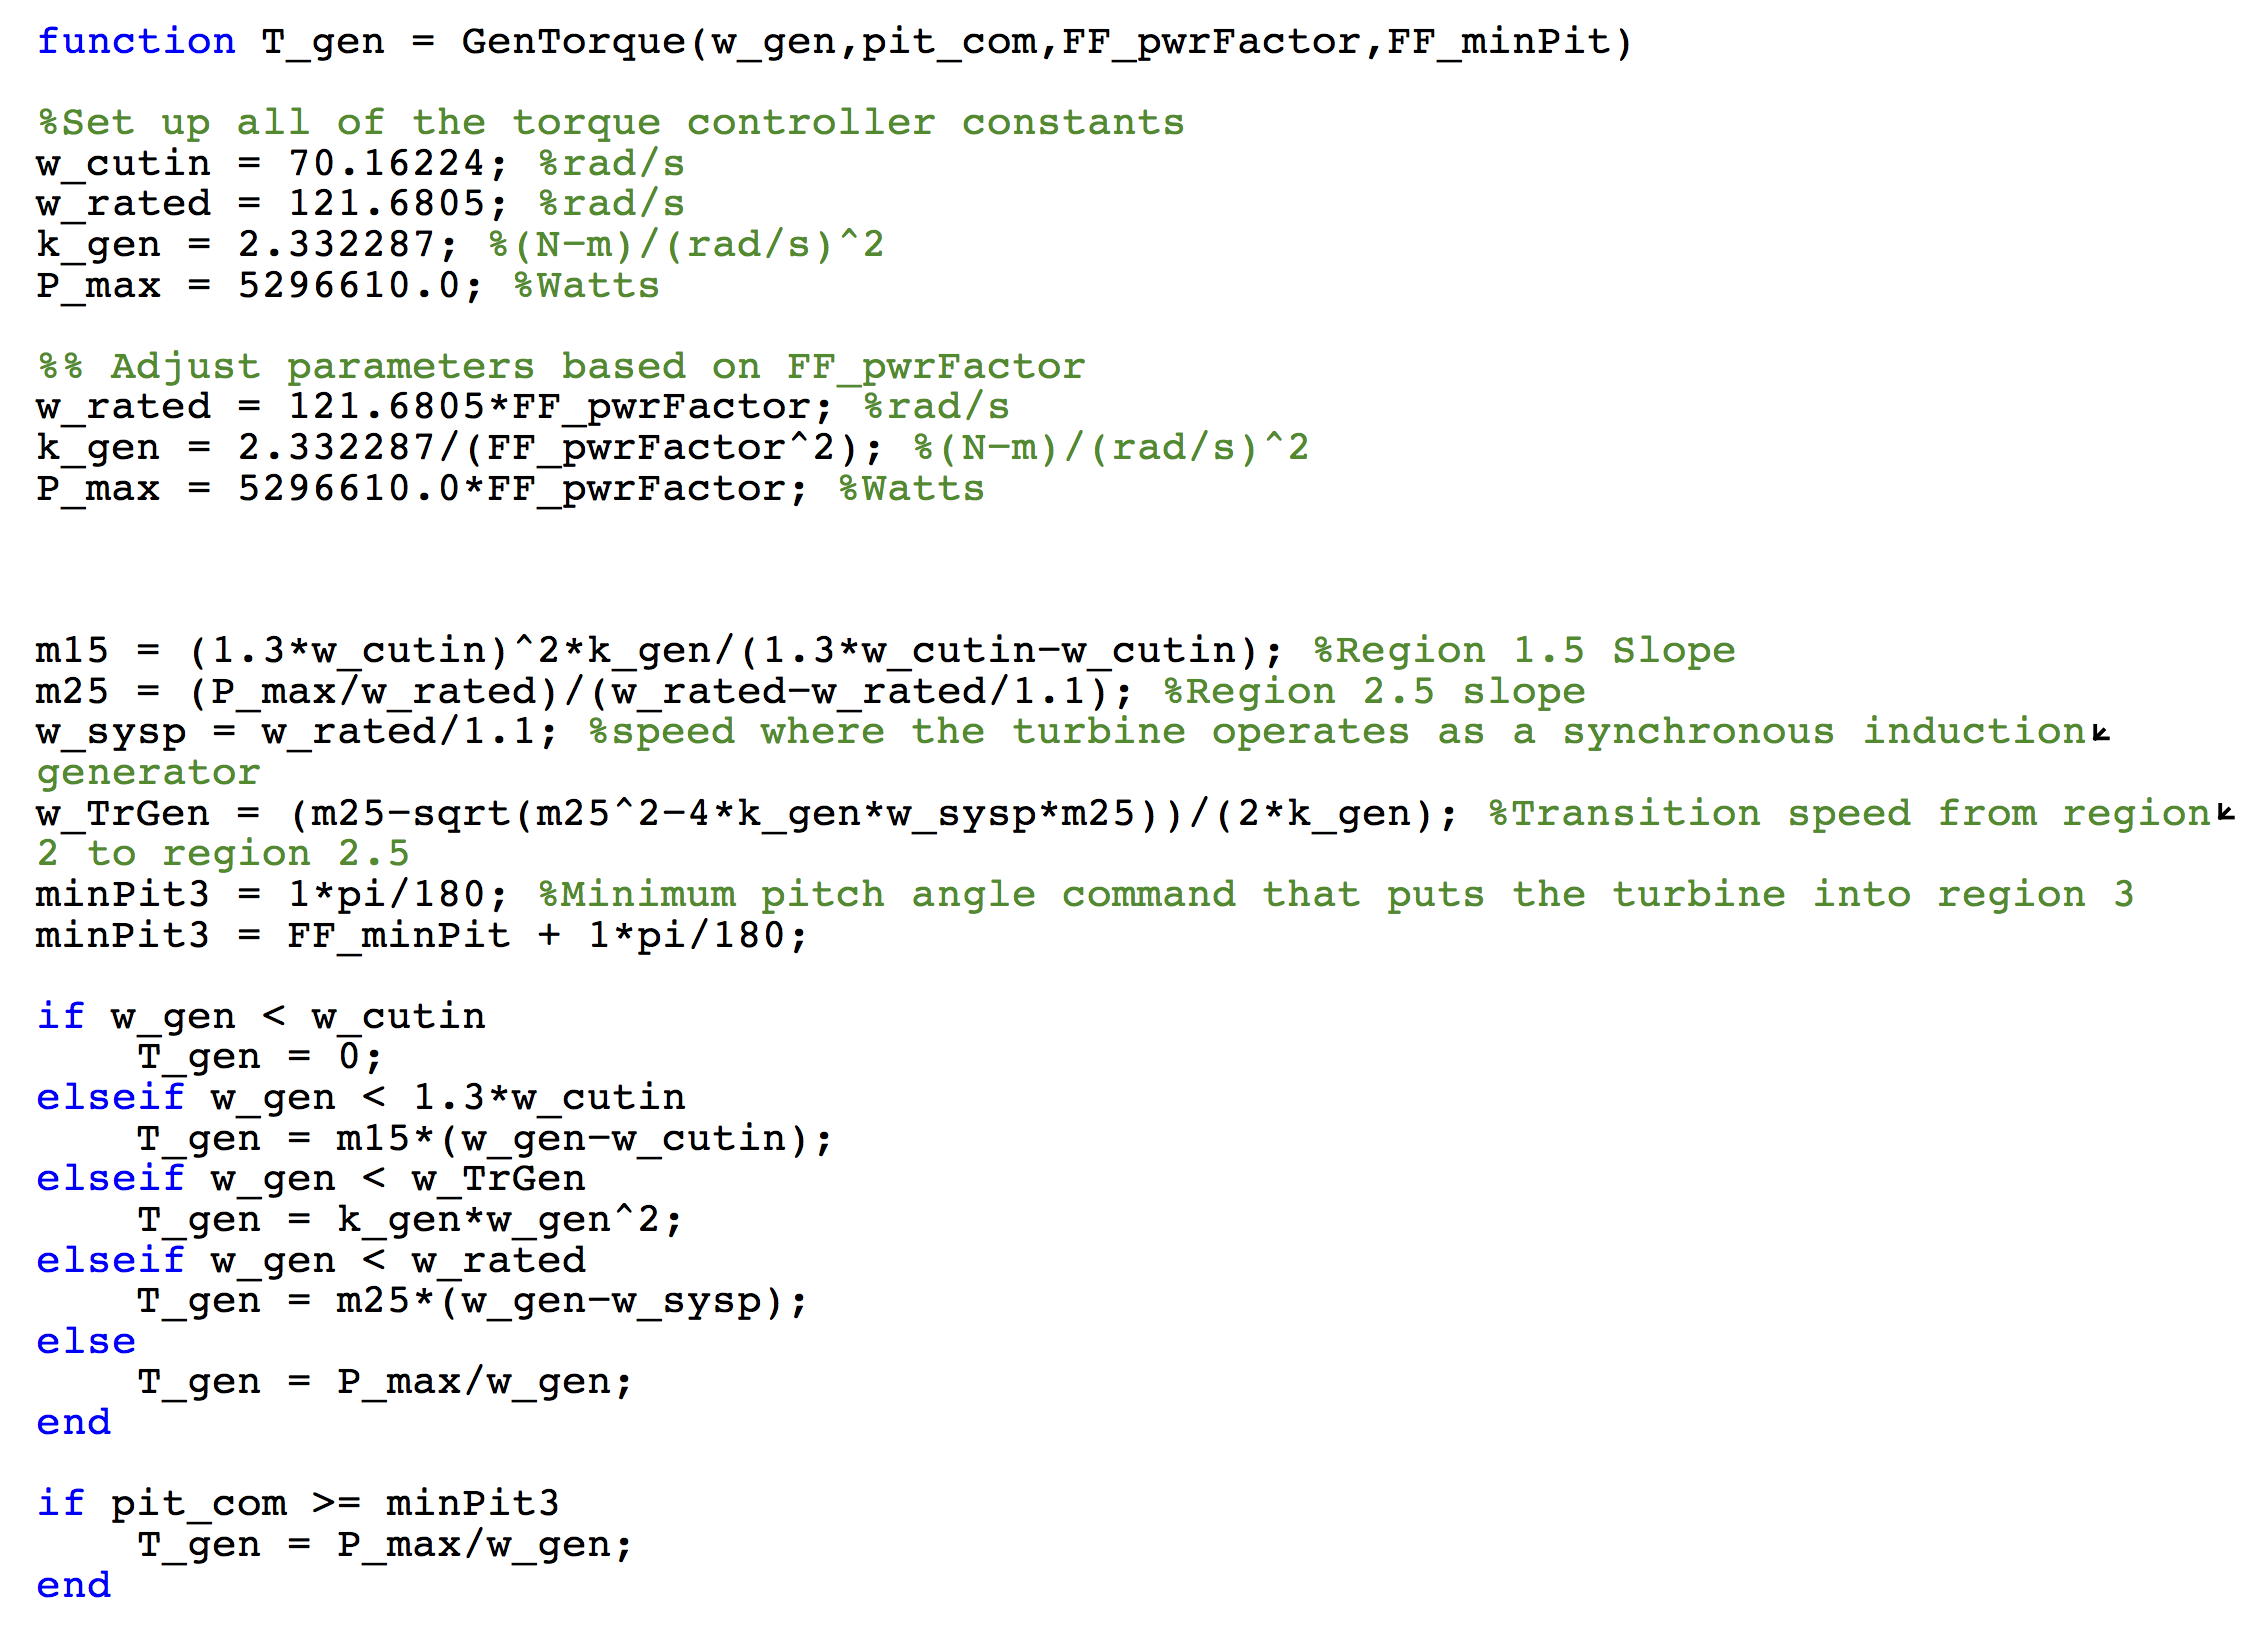
\includegraphics[width=\linewidth]{Figures/AppendixBFigures/FF_Derate9.png}
	\caption{Embedded Matlab function GenTorque for feed forward derating control.}
	\label{figB-15}
\end{figure}
